\chapter{\textsuperscript{TC3} Respuesta en Frecuencia y Resonancia}\label{chap:respuesta_frecuencia}

\section{Respuesta en Frecuencia}


\begin{itemize}
\item Hasta ahora hemos analizado circuitos alimentados por generadores con frecuencia constante.
\item El análisis de la \textbf{respuesta en frecuencia} consiste en variar la frecuencia de alimentación y estudiar la respuesta.
\item Este análisis se realiza en \textbf{régimen permanente} con señales sinusoidales.
\end{itemize}

\begin{enumerate}
\item Respuesta en Frecuencia
\label{sec:org4955c1c}
La respuesta en frecuencia de un circuito es la variación del comportamiento del circuito a los cambios de la frecuencia de alimentación.
\end{enumerate}


\subsection{Función de Transferencia}

\[
  \fasor{H} = \frac{\fasor{Y}}{\fasor{X}}
\]
\begin{center}
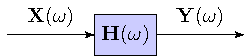
\includegraphics[height=4cm]{../figs/TransferFunction.pdf}
\end{center}


\begin{enumerate}
\item \hfill{}\textsc{BMCOL}
\label{sec:orge6450a2}
\begin{center}
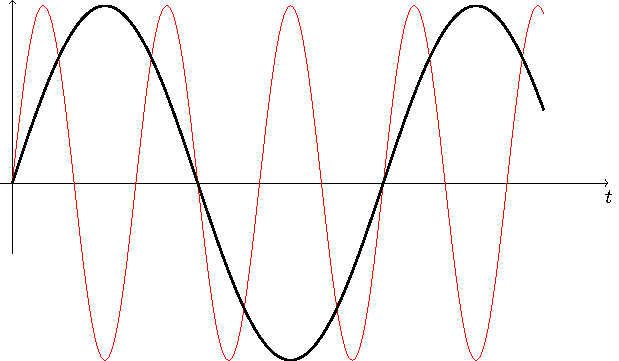
\includegraphics[height=4cm]{../figs/sinX.pdf}
\end{center}

\item \hfill{}\textsc{BMCOL}
\label{sec:org4f673b6}
\begin{center}
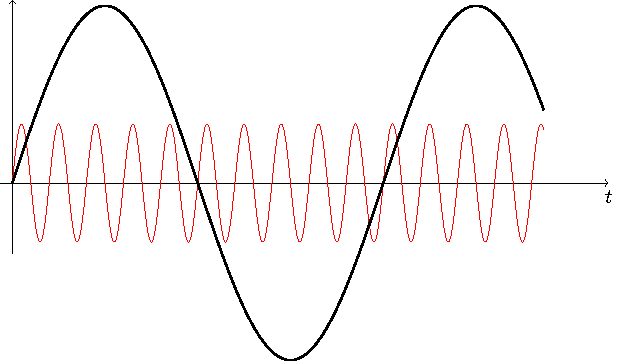
\includegraphics[height=4cm]{../figs/sinY.pdf}
\end{center}
\end{enumerate}


\begin{itemize}
\item Ganancia de Tensión
\end{itemize}
\[
\fasor{H} =\frac{\fasor{V_o}}{\fasor{V_i}}
\]
\begin{itemize}
\item Ganancia de Corriente
\end{itemize}
\[
\fasor{H} =\frac{\fasor{I_o}}{\fasor{I_i}}
\]
\begin{itemize}
\item Impedancia de Transferencia
\end{itemize}
\[
\fasor{H} =\frac{\fasor{V_o}}{\fasor{I_i}}
\]
\begin{itemize}
\item Admitancia de Transferencia
\end{itemize}
\[
\fasor{H} =\frac{\fasor{I_o}}{\fasor{V_i}}
\]

{La función de transferencia es un fasor}
\label{sec:orgd97d35b}

\begin{itemize}
\item Evaluamos la función de transferencia en el eje imaginario:
\end{itemize}
\[
\laplace{H}\rvert_{\slp = j\omega} = \fasor{H} 
\]
\begin{itemize}
\item Dado que estamos en régimen permanente sinusoidal es \textbf{un fasor con módulo y ángulo}:
\end{itemize}
\[
\fasor{H} = H\phase{\phi}
\]

\begin{itemize}
\item Tanto el módulo como el ángulo \textbf{varían con la frecuencia}:
\end{itemize}

\[
\fasor{H} \Rightarrow
\begin{cases} 
  |\fasor{H}|\\
  \phi(\omega)
\end{cases}
\]


\subsection{División de Polinomios: Polos y Ceros}
\label{sec:org4eaf2b1}

\[
  \boxed{\laplace{H}\rvert_{\slp = j\omega} = \frac{\laplace{N}}{\laplace{D}}\rvert_{\slp = j\omega} = K \frac{(\slp-z_1) (\slp - z_2) \ldots (\slp - z_m)}{(\slp-p_1) (\slp - p_2) \ldots (\slp - p_n)}\rvert_{\slp = j\omega} }
\]
\begin{enumerate}
\item \hfill{}\textsc{BMCOL}
\label{sec:org2752e54}
\[
\fasor{H} = \frac{j\omega - \mathbf{z_1}}{(j\omega - \mathbf{p_1}) \cdot (j\omega - \mathbf{p_2})}
\]
\item \hfill{}\textsc{BMCOL}
\label{sec:org1276689}
\begin{center}
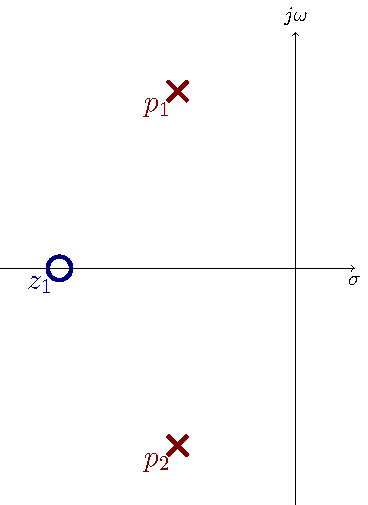
\includegraphics[height=4cm]{../figs/InterpretacionGeometrica0.pdf}
\end{center}
\end{enumerate}

{Interpretación Geométrica}
\label{sec:org5b132e1}

Cada uno de los factores de \(\fasor{H}\) es un número complejo que conecta un cero/polo con el eje imaginario.
\begin{enumerate}
\item \hfill{}\textsc{BMCOL}
\label{sec:org34bdb21}
\[
\fasor{H} = \frac{j\omega - \mathbf{z_1}}{(j\omega - \mathbf{p_1}) \cdot (j\omega - \mathbf{p_2})}
\]
\item \hfill{}\textsc{BMCOL}
\label{sec:orga6ed099}
\begin{center}
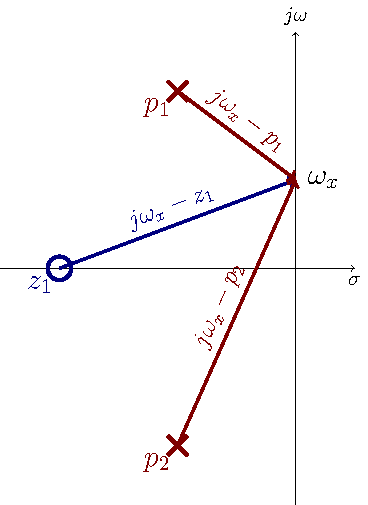
\includegraphics[height=4cm]{../figs/InterpretacionGeometrica.pdf}
\end{center}
\end{enumerate}

{Interpretación Geométrica: cero simple}
\label{sec:org4228a1a}

\[
  \fasor{H} = K \cdot (j\omega - \mathbf{z_1})
\]

\begin{enumerate}
\item \hfill{}\textsc{BMCOL}
\label{sec:orgec55405}
\begin{center}
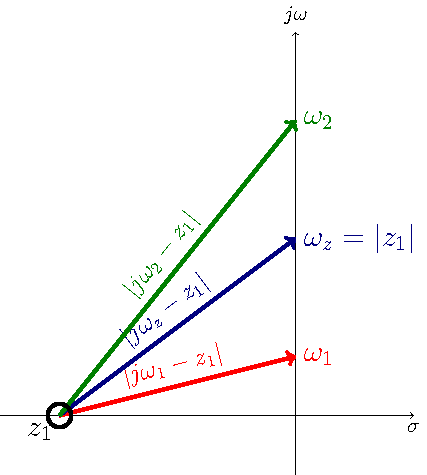
\includegraphics[height=4cm]{../figs/CeroGeometrica.pdf}
\end{center}

\item \hfill{}\textsc{BMCOL}
\label{sec:org876b952}
\begin{center}
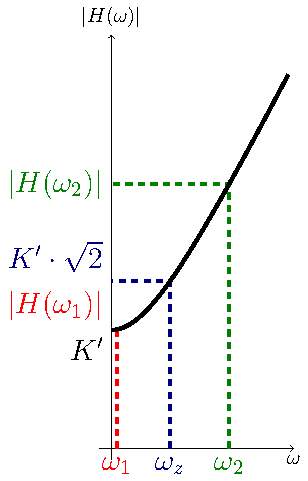
\includegraphics[height=4cm]{../figs/CeroGeometricaPlot.pdf}
\end{center}
\end{enumerate}

{Interpretación Geométrica: polo simple}
\label{sec:orge2be957}

\[
  \fasor{H} = \frac{K}{j\omega - \mathbf{p_1}}
\]

\begin{enumerate}
\item \hfill{}\textsc{BMCOL}
\label{sec:org056cb29}
\begin{center}
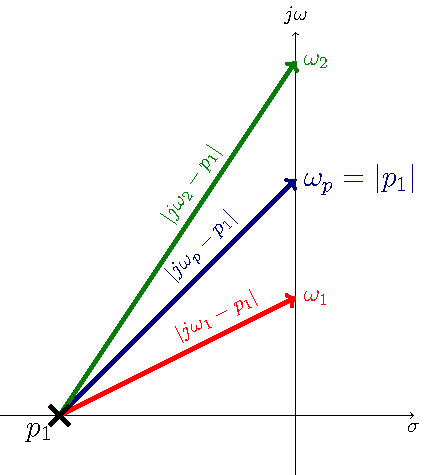
\includegraphics[height=4cm]{../figs/PoloGeometrica.pdf}
\end{center}

\item \hfill{}\textsc{BMCOL}
\label{sec:org05737f5}
\begin{center}
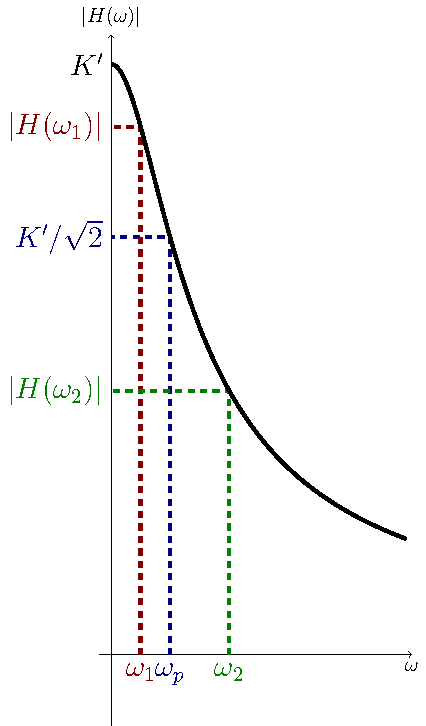
\includegraphics[height=4cm]{../figs/PoloGeometricaPlot.pdf}
\end{center}
\end{enumerate}

{Forma normalizada o estándar}
\label{sec:orgd549f3c}
Para la construcción del diagrama de Bode es conveniente escribir la función en forma normalizada:

\[
  \laplace{H} = K' \frac{(1 + \slp/\omega_{z1}) \cdot (1 + \slp/\omega_{z2}) \ldots (1 + \slp/\omega_{zm})}{(1 + \slp/\omega_{p1}) \cdot (1 + \slp/\omega_{p2}) \ldots (1 + \slp/\omega_{pn})} 
\]

siendo \(\omega\)\textsubscript{zi} y \(\omega\)\textsubscript{pi} las pulsaciones de los ceros y polos, respectivamente.

\subsubsection{Ejercicios Recomendados}
\label{sec:org3a18fb7}
\begin{itemize}
\item AS: Ejemplo 14.2.
\item Exámenes:
\begin{itemize}
\item Feb 2004 (a), Jun 2013 (a)
\item Sep 2007 (a), Feb 2005 (a), Feb 2010 (a)
\item Nov 2014 (a), Sep 2005 (a), Sep 2006 (a).
\end{itemize}
\end{itemize}

\subsection{Diagrama de Bode}
\label{sec:org9b5c0f5}


\begin{itemize}
\item Un diagrama de Bode representa de forma \textbf{aproximada} la magnitud y la fase de la función de transferencia.
\item Son \textbf{gráficos semilogarítmicos}:
\begin{itemize}
\item Magnitud en \textbf{decibelios} frente al logaritmo de la frecuencia/pulsación.
\item Fase en radianes/grados frente al logaritmo de la frecuencia/pulsación.
\end{itemize}
\end{itemize}
\begin{center}
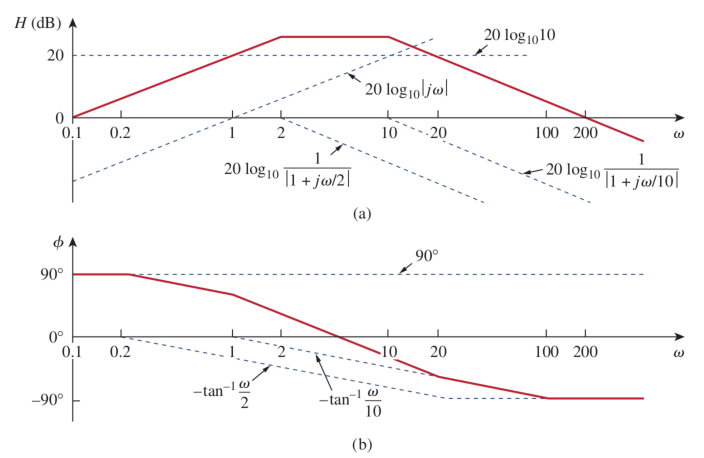
\includegraphics[height=4cm]{../figs/Bode.pdf}
\end{center}

{Repaso de logaritmos}

\begin{enumerate}
\item Propiedades
\label{sec:org9103f67}
\begin{align*}
  \log (P_1 \cdot P_2) &= \log P_1 + \log P_2\\
  \log \frac{P_1}{P_2} &= \log P_1 - \log P_2\\
  \log P^n &= n \cdot \log P
\end{align*}

\item Valores útiles
\label{sec:orge81bc9a}
\[
\begin{array}{ll}
  \log 1 = 0 & \log 2 = 0.30103\\
  \log 10 = 1 & \log \frac{1}{2} = -0.30103
\end{array}
\]
\end{enumerate}

{Decibelio}


El \textbf{decibelio} (\(\si{\decibel}\)) se emplea para medir la ganancia de potencia o la ratio de dos niveles de potencia:

\[
G_{dB} = 10 \log G = 10 \log \frac{P_2}{P_1}
\]
\begin{center}
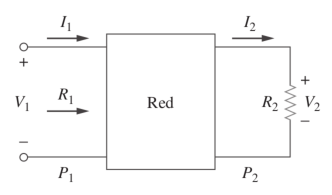
\includegraphics[height=4cm]{../figs/Red_Ganancia.pdf}
\end{center}



Suponiendo \(R_1 = R_2\), también se emplea para medir la ganancia de tensión/corriente:

\[
G_{dB} = 10 \log \frac{V_2^2}{V_1^2} = 20 \log \frac{V_2}{V_1}
\]
\begin{center}
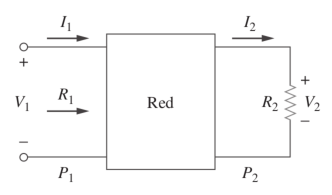
\includegraphics[height=4cm]{../figs/Red_Ganancia.pdf}
\end{center}

{Valores importantes}

\begin{itemize}
\item Ganancia unidad
\end{itemize}

\[
  G = 1 \Rightarrow
  \left\{
  \begin{array}{c}
    P_1 = P_2\\
    \\
    V_1 = V_2
  \end{array}
  \right\}
  \Rightarrow
  \left\{
  \begin{array}{c}
    G_{dB} = 10 \log \frac{P_2}{P1} = \SI{0}{\decibel}\\
    \\
    G_{dB} = 20 \log \frac{V_2}{V1} = \SI{0}{\decibel}
  \end{array}
  \right\}
\]

\begin{itemize}
\item Potencia Mitad
\end{itemize}

\[
  P_2 = \frac{P_1}{2} \Rightarrow
  \left\{
  \begin{array}{c}
    G = \frac{1}{2}\\
    \\
    V_2 = \frac{V_1}{\sqrt{2}}
  \end{array}
  \right\}
  \Rightarrow
  \left\{
  \begin{array}{c}
    G_{dB} = 10 \log \frac{P_2}{P1} = -\SI{3}{\decibel}\\
    \\
    G_{dB} = 20 \log \frac{V_2}{V_1} = -\SI{3}{\decibel}
  \end{array}
  \right\}
\]

{Construcción del Diagrama de Bode}
\begin{itemize}
\item Reescribimos \(\laplace{H}\) de forma normalizada
\end{itemize}
\[
  \laplace{H}\rvert_{\slp =j\omega} = K \frac{(1 + \slp/\omega_{z1}) \cdot (1 + \slp/\omega_{z2}) \ldots (1 + \slp/\omega_{zm})}{(1 + \slp/\omega_{p1}) \cdot (1 + \slp/\omega_{p2}) \ldots (1 + \slp/\omega_{pn})} 
\]
\begin{itemize}
\item Módulo
\end{itemize}
\[
  |\fasor{H}| = K \frac{|1 + j\omega/\omega_{z1}| \cdot |1 + j\omega/\omega_{z2}| \ldots |1 + j\omega/\omega_{zm}|}{|1 + j\omega/\omega_{p1}| \cdot |1 + j\omega/\omega_{p2}| \ldots |1 + j\omega/\omega_{pn}|} 
\]

\begin{itemize}
\item Ángulo
\end{itemize}
\begin{align*}
\phi(\omega) &= \atan(\omega/\omega_{z1}) + \atan(\omega/\omega_{z2}) + \ldots + \atan(\omega/\omega_{zm}) - \\
&- \left(\atan(\omega/\omega_{p1}) + \atan(\omega/\omega_{p2}) + \ldots + \atan(\omega/\omega_{pn})\right) 
\end{align*}


\begin{itemize}
\item Al aplicar logaritmos a la expresión de la amplitud \textbf{los productos se convierten en sumas}.
\item La estrategia de construcción consiste en analizar la \textbf{contribución de cada cero/polo por separado} y \textbf{sumar} para obtener el resultado global.
\end{itemize}

\begin{center}
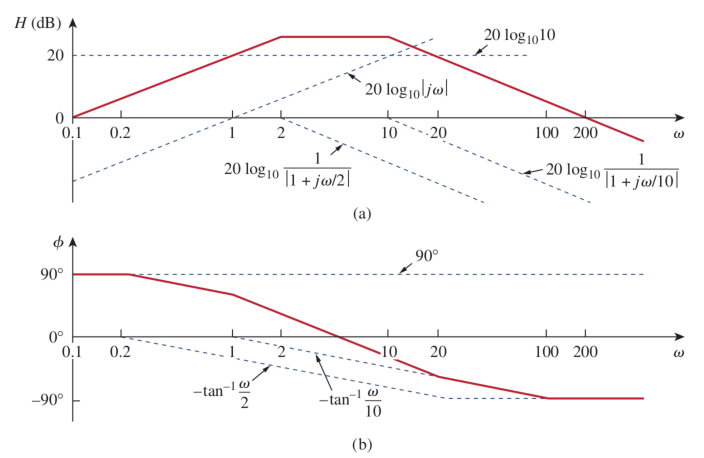
\includegraphics[height=4cm]{../figs/Bode.pdf}
\end{center}


\begin{enumerate}
\item Posibilidades
\begin{itemize}
\item Término constante: \(K\)
\item Cero/Polo en el origen: \(j\omega\)
\item Cero/Polo simple: \(1 + j\omega/\omega_c\)
\item Cero/Polo múltiple (\emph{raíces reales repetidas}): \((1 + j\omega/\omega_c)^N\)
\item Cero/Polo cuadrático (\emph{raíces complejas conjugadas}): \(1 - (\omega/\omega_0)^2 + j2\zeta\omega/\omega_0\)
\end{itemize}
\end{enumerate}

{Término Constante}

\[
  \fasor{H} = K \Rightarrow
  \begin{cases}
    |\fasor{H}| = 20 \log |K|\\
    \phi(\omega) = 
    \begin{cases}
      \ang{0} \quad si \quad K > 0\\
      \ang{180} \quad si \quad K < 0\\
    \end{cases}
  \end{cases}
\]

\begin{center}
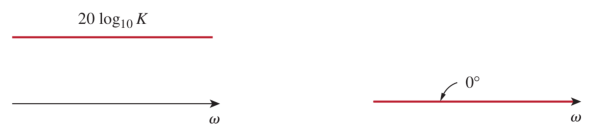
\includegraphics[height=4cm]{../figs/BodeConstante.pdf}
\end{center}

{Cero en el origen}

\textbf{Atención}: el origen \(\omega = 0\) no se representa en una escala logarítmica.
\label{sec:org10a2611}
\[
  \fasor{H} = j\omega \Rightarrow
  \begin{cases}
    |\fasor{H}| = 20 \log \omega\\
    \phi(\omega) = \ang{90}
  \end{cases}
\]



\begin{center}
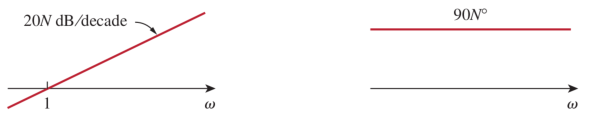
\includegraphics[height=4cm]{../figs/BodeCeroOrigen.pdf}
\end{center}

Década: rango de frecuencias comprendido entre \(\omega_1\) y \(10\cdot\omega_1\).

{Polo en el origen}
\[
  \fasor{H} = \frac{1}{j\omega} \Rightarrow
  \begin{cases}
    |\fasor{H}| = - 20 \log \omega\\
    \phi(\omega) = - \ang{90}
  \end{cases}
\]

\begin{center}
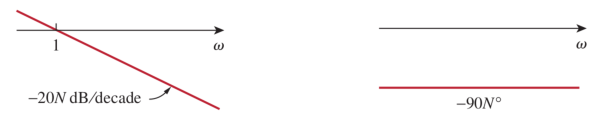
\includegraphics[height=4cm]{../figs/BodePoloOrigen.pdf}
\end{center}

{Cero simple}


\[
  \fasor{H} = 1 + j\frac{\omega}{\omega_z} \Rightarrow
  \begin{cases}
    |\fasor{H}| =  20 \log \sqrt{1 + \left(\frac{\omega}{\omega_z}\right)^2}\\
    \phi(\omega) = \atan(\frac{\omega}{\omega_z}) 
  \end{cases}
\]

\begin{enumerate}
\item \hfill{}\textsc{BMCOL}
\label{sec:org18a1aae}
\[
  |\fasor{H}| = 
  \begin{cases}
  20 \log 1 = 0, \enskip \omega \to 0\\
  20 \log \frac{\omega}{\omega_z}, \enskip \omega \gg \omega_z\\
  \end{cases}
\]

\item \hfill{}\textsc{BMCOL}
\label{sec:orgff9fa7c}
\[
  \phi(\omega) = 
  \begin{cases}
    \ang{0},\enskip \omega \leq 0.1\omega_z\\
    \ang{45}, \enskip \omega = \omega_z\\
    \ang{90}, \enskip \omega \geq 10\omega_z\\
  \end{cases}
\]

\item \hfill{}\textsc{B\_ignoreheading}
\label{sec:org66bf0da}
\begin{center}
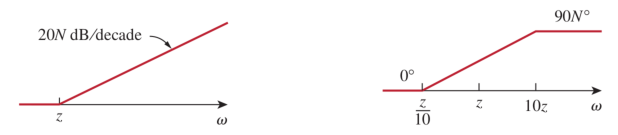
\includegraphics[height=4cm]{../figs/BodeCeroSimple.pdf}
\end{center}
\end{enumerate}

{Polo simple}

\[
  \fasor{H} = \frac{1}{1 + j\frac{\omega}{\omega_p}} \Rightarrow
  \begin{cases}
    |\fasor{H}| =  - 20 \log \sqrt{1 + \left(\frac{\omega}{\omega_p}\right)^2}\\
    \phi(\omega) = - \atan(\frac{\omega}{\omega_p}) 
  \end{cases}
\]

\begin{enumerate}
\item \hfill{}\textsc{BMCOL}
\label{sec:org9ce6f1c}
\[
  |\fasor{H}| = 
  \begin{cases}
  - 20 \log 1 = 0, \enskip \omega \to 0\\
  - 20 \log \frac{\omega}{\omega_p}, \enskip \omega \gg \omega_p\\
  \end{cases}
\]

\item \hfill{}\textsc{BMCOL}
\label{sec:org1fb87ac}
\[
  \phi(\omega) = 
  \begin{cases}
    \ang{0},\enskip \omega \leq 0.1\omega_p\\
    - \ang{45}, \enskip \omega = \omega_p\\
    - \ang{90}, \enskip \omega \geq 10 \omega_p
  \end{cases}
\]

\item \hfill{}\textsc{B\_ignoreheading}
\label{sec:org46bb3bd}
\begin{center}
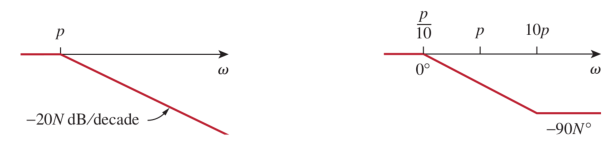
\includegraphics[height=4cm]{../figs/BodePoloSimple.pdf}
\end{center}
\end{enumerate}

{Cero cuadrático}

Sea \(\laplace{H}\rvert_{\slp = j\omega}  = \slp^2 + 2\alpha \slp + \omega_0^2\), con \(\alpha < \omega_0\). Usando \(\zeta = \alpha/\omega_0 < 1\) y normalizando:

\[
  \fasor{H} = 1 + j 2 \zeta \frac{\omega}{\omega_0} - \left(\frac{\omega}{\omega_0}\right)^2 
\]

\begin{enumerate}
\item \hfill{}\textsc{BMCOL}
\label{sec:org4e9c2ca}
\[
  |\fasor{H}| = 
  \begin{cases}
  0, \enskip \omega \to 0\\
  40 \log (\omega/\omega_0), \enskip \omega \gg \omega_0\\
  \end{cases}
\]

\item \hfill{}\textsc{BMCOL}
\label{sec:orgd9fd893}
\[
  \phi(\omega) = 
  \begin{cases}
    \ang{0},\enskip \omega \leq 0.1\omega_0\\
    \ang{90}, \enskip \omega = \omega_0\\
    \ang{180}, \enskip \omega \geq 10 \omega_0
  \end{cases}
\]

\item \hfill{}\textsc{B\_ignoreheading}
\label{sec:orga137928}
\begin{center}
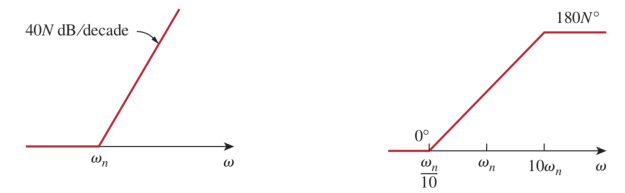
\includegraphics[height=4cm]{../figs/BodeCeroCuadratico.pdf}
\end{center}
\end{enumerate}


{Polo cuadrático}

\[
  \fasor{H} = \frac{1}{1 + j 2 \zeta \frac{\omega}{\omega_0} - \left(\frac{\omega}{\omega_0}\right)^2} 
\]

\begin{enumerate}
\item \hfill{}\textsc{BMCOL}
\label{sec:orgaafc65d}
\[
  |\fasor{H}| = 
  \begin{cases}
  0, \enskip \omega \to 0\\
  - 40 \log (\omega/\omega_0), \enskip \omega \gg \omega_0\\
  \end{cases}
\]

\item \hfill{}\textsc{BMCOL}
\label{sec:org5f23b3a}
\[
  \phi(\omega) = 
  \begin{cases}
    \ang{0},\enskip \omega \leq 0.1\omega_0\\
    - \ang{90}, \enskip \omega = \omega_0\\
    - \ang{180}, \enskip \omega \geq 10 \omega_0
  \end{cases}
\]


\item \hfill{}\textsc{B\_ignoreheading}
\label{sec:org6121336}
\begin{center}
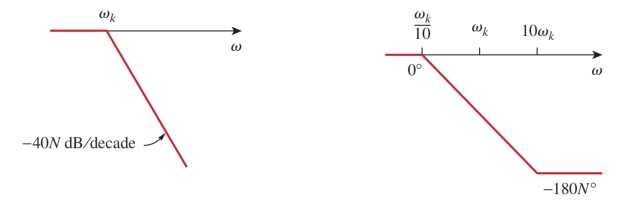
\includegraphics[height=4cm]{../figs/BodePoloCuadratico.pdf}
\end{center}
\end{enumerate}

\subsubsection{Ejercicios Recomendados}
\begin{itemize}
\item AS: ejemplos 14.3, 14.4, 14.5, 14.6.
\item Exámenes:
\begin{itemize}
\item Feb 2004 (b), Jun 2013 (b)
\item Sep 2007 (b), Feb 2005 (b), Feb 2010 (b)
\item Nov 2014 (b), Sep 2005 (b), Sep 2006 (b).
\end{itemize}
\end{itemize}

\subsection{Filtros}

{Filtro Paso Bajo}
\begin{enumerate}
\item \hfill{}\textsc{BMCOL}

\begin{align*}
  |H(0)| &= 1\\
  |H(\omega_c)| &= 1/\sqrt{2}\\
  |H(\infty)| &= 0
\end{align*}

\begin{center}
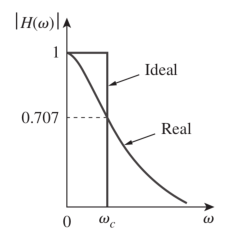
\includegraphics[height=4cm]{../figs/Filtro_PasoBajo.pdf}
\end{center}
\end{enumerate}

{Filtro Paso Alto}


\begin{align*}
  |H(0)| &= 0\\
  |H(\omega_c)| &= 1/\sqrt{2}\\
  |H(\infty)| &= 1
\end{align*}


\begin{center}
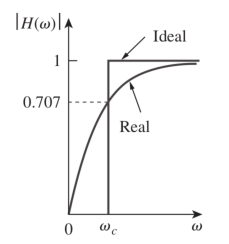
\includegraphics[height=4cm]{../figs/Filtro_PasoAlto.pdf}
\end{center}

{Filtro Paso Banda}

\begin{align*}
  |H(\omega < \omega_1)| &= 0\\
  |H(\omega_1 < \omega < \omega_2)| &= 1\\
  |H(\omega > \omega_2)| &= 0
\end{align*}

\begin{center}
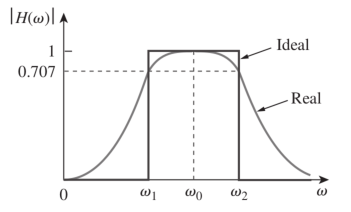
\includegraphics[height=4cm]{../figs/Filtro_PasoBanda.pdf}
\end{center}

{Filtro Banda Eliminada}

\begin{align*}
  |H(\omega < \omega_1)| &= 1\\
  |H(\omega_1 < \omega < \omega_2)| &= 0\\
  |H(\omega > \omega_2)| &= 1
\end{align*}

\begin{center}
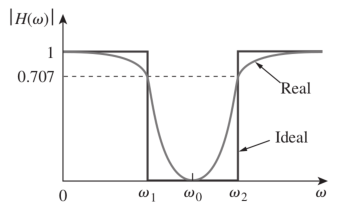
\includegraphics[height=4cm]{../figs/Filtro_BandaEliminada.pdf}
\end{center}

{Ejemplo: circuito RC}

\begin{center}
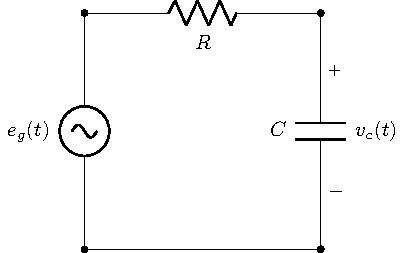
\includegraphics[height=4cm]{../figs/filtroRC.pdf}
\end{center}

\begin{center}
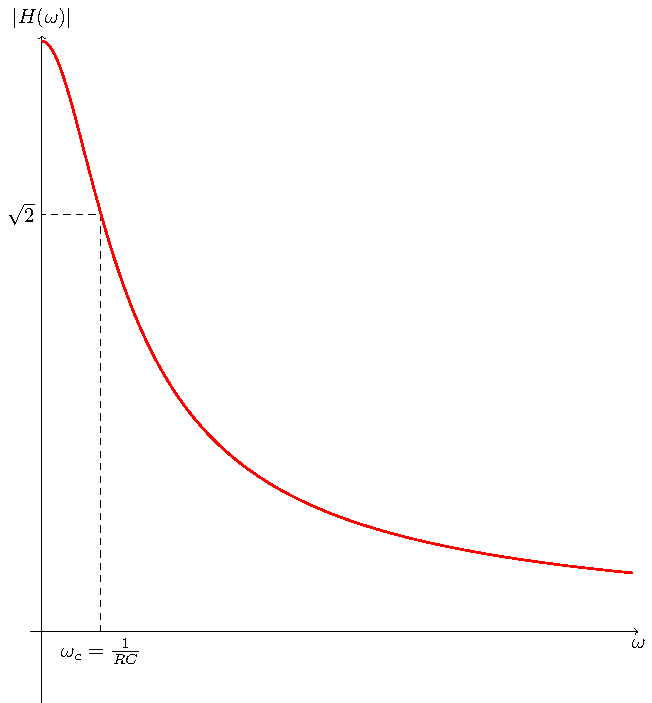
\includegraphics[height=4cm]{../figs/Hw_RC.pdf}
\end{center}

\[
\laplace{H} = \frac{\laplace{U_c}}{\laplace{E_g}} \Rightarrow |\fasor{H}| = \frac{1}{\sqrt{1 + (\omega/\omega_c)^2}} 
\]

{Ejemplo: circuito RL}

\begin{center}
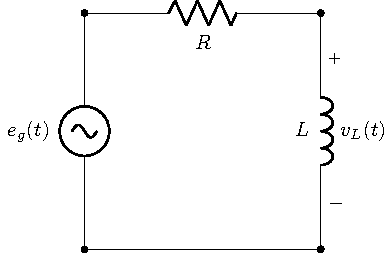
\includegraphics[height=4cm]{../figs/filtroRL.pdf}
\end{center}

\begin{center}
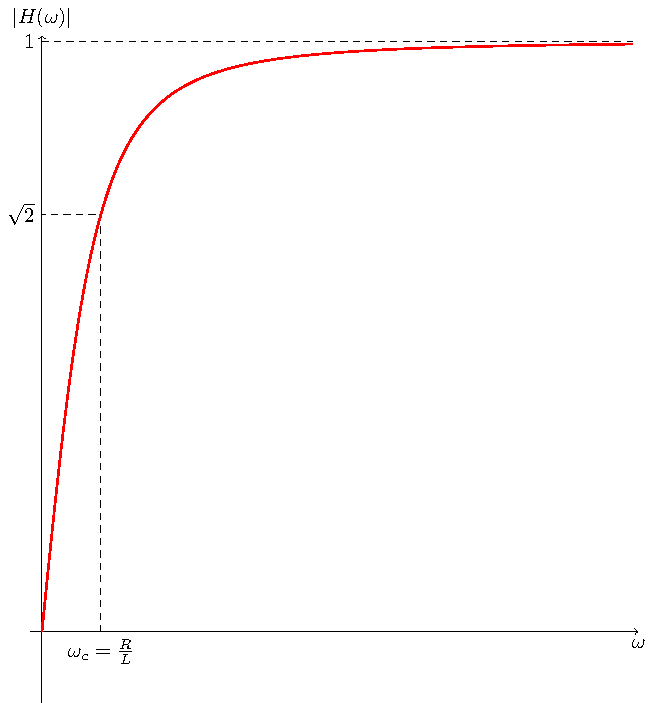
\includegraphics[height=4cm]{../figs/Hw_RL.pdf}
\end{center}

\[
\laplace{H} = \frac{\laplace{U_L}}{\laplace{E_g}} \Rightarrow |\fasor{H}| = \frac{\omega/\omega_c}{\sqrt{1 + (\omega/\omega_c)^2}} 
\]

\subsubsection{Circuitos para practicar}
\label{sec:org68b69b1}


\[
  \fasor{H} = \frac{\fasor{U_R}}{\fasor{E_g}}
\]
\begin{center}
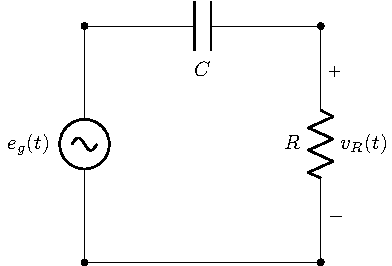
\includegraphics[height=4cm]{../figs/filtroCR.pdf}
\end{center}

\[
  \fasor{H} = \frac{\fasor{U_R}}{\fasor{E_g}}
\]
\begin{center}
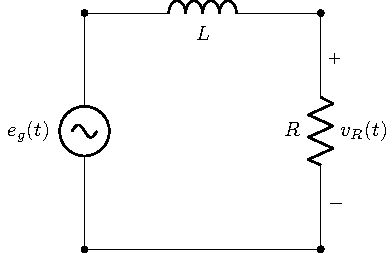
\includegraphics[height=4cm]{../figs/filtroLR.pdf}
\end{center}


\section{Resonancia}
\label{sec:org4ff37ef}
\subsection{Definición}
\label{sec:org004e9ed}
\begin{itemize}
\item Cuando un circuito eléctrico está en resonancia:
\begin{itemize}
\item La \textbf{parte imaginaria} de su impedancia/admitancia es \textbf{nula}.
\item La \textbf{tensión y corriente} están en \textbf{fase}.
\item La \textbf{potencia reactiva} neta es \textbf{nula}.
\end{itemize}
\item La resonancia se produce en una \textbf{frecuencia determinada}, \(f_0\).
\item Sólo puede ocurrir en circuitos con \textbf{al menos un inductor y un capacitor}.
\end{itemize}

{Ancho de Banda y Factor de Calidad}

\begin{itemize}
\item Frecuencias de potencia mitad: \(\omega_1, \omega_2\)
\end{itemize}
\begin{align*}
  |\fasor{Z}|_{\omega = \omega_{1,2}} &=  \frac{1}{\sqrt{2}}\cdot |\mathbf{Z}(\omega_0)|\\
  |\fasor{Y}|_{\omega = \omega_{1,2}} &=  \frac{1}{\sqrt{2}}\cdot |\mathbf{Y}(\omega_0)|
\end{align*}
\begin{center}
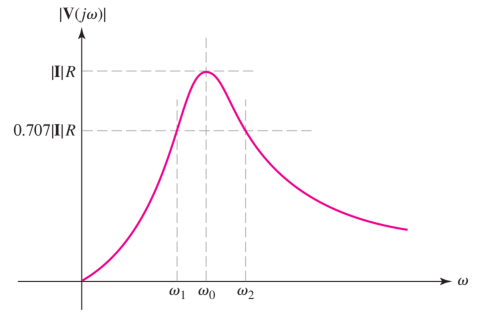
\includegraphics[width=.9\linewidth]{../figs/CurvaResonancia.pdf}
\end{center}

\begin{itemize}
\item Ancho de Banda (\emph{de potencia mitad}):
\end{itemize}
\[
  B = \omega_2 - \omega_1
\]

\begin{itemize}
\item Factor de Calidad (\emph{en resonancia}):
\end{itemize}
\[
  \boxed{Q_0 = \frac{\omega_0}{B}}
\]


\begin{center}
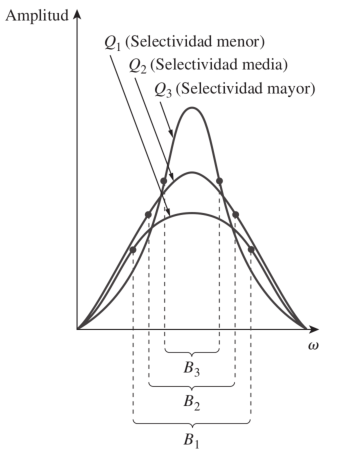
\includegraphics[height=4cm]{../figs/Q_B.pdf}
\end{center}
\subsection{Circuito RLC paralelo}
\label{sec:orgab7f8ca}


{Admitancia}

\begin{center}
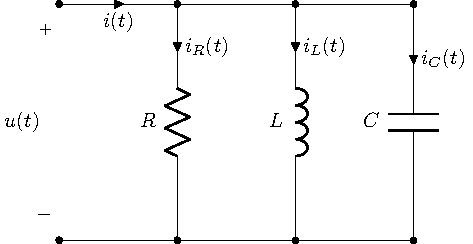
\includegraphics[height=4cm]{../figs/RLC_paralelo_resonante.pdf}
\end{center}

\begin{itemize}
\item Admitancia:
\end{itemize}
\[
  \fasor{Y} = \frac{1}{R} + j(\omega C - \frac{1}{\omega L})
\]
\begin{itemize}
\item Módulo en resonancia \(\omega_0\):
\end{itemize}
\[
  |\mathbf{Y}(\omega_0)| = \frac{1}{R} \rightarrow \omega_0 C - \frac{1}{\omega_0 L} = 0
\]

\[
  \boxed{\omega_0 = \frac{1}{\sqrt{LC}}}
\]

{Puntos de Potencia Mitad}

\begin{itemize}
\item Definición de Puntos de potencia mitad (\(\omega_1, \omega_2\))
\end{itemize}
\begin{align*}
|\mathbf{Y}(\omega_1)| &= \frac{1}{\sqrt{2} R} \xrightarrow{\textcolor{blue}{\omega_1 < \omega_0}} \omega_1 C - \frac{1}{\omega_1 L} = \textcolor{blue}{-}\frac{1}{R}\\
|\mathbf{Y}(\omega_2)| &= \frac{1}{\sqrt{2} R} \xrightarrow{\textcolor{blue}{\omega_2 > \omega_0}} \omega_2 C - \frac{1}{\omega_2 L} =  \textcolor{blue}{+}\frac{1}{R}
\end{align*}

\begin{itemize}
\item Ecuaciones
\end{itemize}
\begin{align*}
  \omega_1^2 \omega_0^2 \textcolor{blue}{+} \frac{\omega_1 L}{R} - 1 &= 0\\
  \omega_2^2 \omega_0^2 \textcolor{blue}{-} \frac{\omega_2 L}{R} - 1 &= 0
\end{align*}

{Ancho de Banda y Factor de Calidad}

\begin{itemize}
\item Resultado
\end{itemize}
\begin{align*}
\omega_1 &= \textcolor{blue}{-}\frac{1}{2RC} + \sqrt{\left(\frac{1}{2RC}\right)^2 + \frac{1}{LC}}\\
\omega_2 &= \textcolor{blue}{+}\frac{1}{2RC} + \sqrt{\left(\frac{1}{2RC}\right)^2 + \frac{1}{LC}}
\end{align*}

\begin{itemize}
\item Ancho de Banda
\end{itemize}
\[
\boxed{B = \omega_2 - \omega_1 = \frac{1}{RC}}
\]

\begin{itemize}
\item Factor de Calidad
\end{itemize}
\[
  \boxed{Q_0 = \frac{\omega_0}{B} = \omega_0 R C = \frac{R}{\omega_0 L}}
\]

{Balance de corrientes en resonancia}

\begin{center}
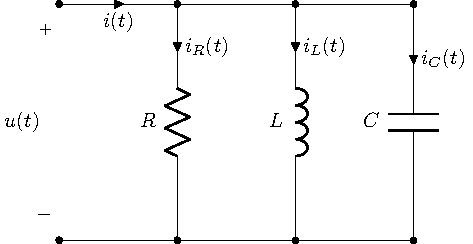
\includegraphics[height=4cm]{../figs/RLC_paralelo_resonante.pdf}
\end{center}

\[
  u(t) = U_0 \sin(\omega_0 t)
\]

\[
\left.
\begin{array}{l}
  i_R(t) = \frac{U_0}{R} \sin(\omega_0 t)\\
  i_L(t) = - \frac{U_0}{\omega_0 L} \cos(\omega_0 t)\\
  i_C(t) = \omega_0 C U_0 \cos(\omega_0 t)
\end{array}
\right\} \xrightarrow{\omega_0 = \frac{1}{\sqrt{LC}}} \boxed{i(t) = i_R(t)}
\]

\begin{center}
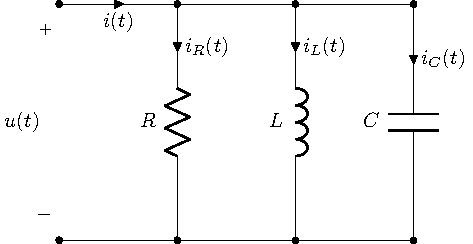
\includegraphics[height=4cm]{../figs/RLC_paralelo_resonante.pdf}
\end{center}

\begin{itemize}
\item Valores máximos (\textbf{atención en circuitos con \(Q\) alto})
\end{itemize}
\[
  I_{R0} = \max\{i_R(t)\} = \frac{U_0}{R}
\]

\[
  I_{L0} = \max\{i_L(t)\} = \frac{U_0}{\omega_0 L} \xrightarrow{Q_0 = \frac{R}{\omega_0L}} \boxed{\frac{I_{L0}}{I_{R0}} = Q_0}
\]

\[
  I_{C0} = \max\{i_C(t)\} = \omega_0 C U_0 \xrightarrow{Q_0 = \omega_0CR} \boxed{\frac{I_{C0}}{I_{R0}} = Q_0}
\]

{Balance de Energías}

\[
  u(t) = U_0 \sin(\omega t)
\]

\begin{itemize}
\item Energías total almacenada en \(\omega \neq \omega_0\):
\end{itemize}
\begin{align*}
  w_L(t) &= \frac{1}{2} L i_L^2(t) = \frac{U_0^2}{2 \omega^2 L} \cos^2 (\omega t)\\
  w_C(t) &= \frac{1}{2} C u^2(t) = \frac{U_0^2 C}{2} \sin^2 (\omega t) \\
  \cline{1-2}
  w_C(t) + w_L(t) &= \frac{U_0^2}{2} \left(C\sin^2(\omega t) + \frac{U_0^2}{2 \omega^2 L} \cos^2(\omega t)\right)
\end{align*}

\begin{itemize}
\item La energía almacenada en resonancia es \textbf{constante}:
\end{itemize}
\[
\omega = \omega_0 = \frac{1}{\sqrt{LC}} \rightarrow \boxed{w_C(t) + w_L(t) = \frac{1}{2} C U_0^2}
\]

{Nueva definición del Factor de Calidad}

\begin{itemize}
\item Energía almacenada en resonancia:
\end{itemize}
\[
w_{total} = \frac{1}{2} C U_0^2 = C U^2
\]

\begin{itemize}
\item Energía disipada en un período
\end{itemize}
\[
P_R = \frac{U^2}{R} \rightarrow w_R = T_0 \cdot \frac{U^2}{R}
\]

\begin{itemize}
\item Ratio entre almacenamiento y disipación
\end{itemize}

\[
\frac{w_{total}}{w_R} = f_0 C R \xrightarrow{Q_0 = \omega_0 C R} \boxed{Q_0 = 2 \pi \frac{w_{total}}{w_R}}
\]

\begin{itemize}
\item Un circuito resonante almacena \(Q_0/2\pi\) veces la energía suministrada.
\end{itemize}

{La curva de resonancia \textbf{no} es simétrica}

La frecuencia de resonancia no está en el centro del ancho de banda
\begin{center}
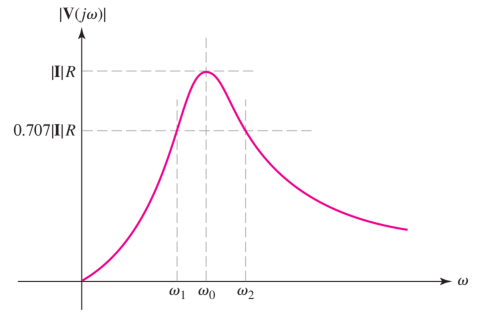
\includegraphics[height=4cm]{../figs/CurvaResonancia.pdf}
\end{center}


\begin{itemize}
\item Retomamos expresión de puntos de potencia mitad:
\end{itemize}
\[
\omega_{1,2} = \sqrt{\left(\frac{1}{2RC}\right)^2 + \frac{1}{LC}} \mp \frac{1}{2RC}
\]

\begin{itemize}
\item Los expresamos en función de \(Q\) y \(\omega_0\):
\end{itemize}

\[
\omega_{1,2}= \omega_0\left(\sqrt{\left(\frac{1}{2Q_0}\right)^2 + 1} \mp \frac{1}{2Q_0}\right)
\]

\begin{itemize}
\item La frecuencia de resonancia es la media geométrica (\emph{no está en el centro del ancho de banda}).
\end{itemize}
\[
  \boxed{\omega_1 \cdot \omega_2 = \omega_0^2} 
\]

{Aproximación para circuitos con alto \(Q_0\)}

\begin{itemize}
\item Cuando \(Q \geq 10\) podemos escribir:
\end{itemize}
\begin{align*}
\omega_1 &\simeq \omega_0\left(1 - \frac{1}{2Q_0}\right) = \omega_0 - \frac{B}{2}\\
\omega_2 &\simeq \omega_0\left(1 + \frac{1}{2Q_0}\right) = \omega_0 + \frac{B}{2}
\end{align*}

\begin{itemize}
\item En circuitos de \textbf{alto factor de calidad}, la frecuencia de resonancia está \textbf{aproximadamente} en el \textbf{centro} del ancho de banda.
\end{itemize}

\[
  \boxed{\omega_0 \simeq \frac{1}{2}(\omega_1 + \omega2)}
\]

{Admitancia en función de \(\omega_0\) y \(Q_0\)}

\begin{itemize}
\item Recordamos expresión de la admitancia:
\end{itemize}

\[
  \fasor{Y} = \frac{1}{R} + j(\omega C - \frac{1}{\omega L})
\]
\begin{itemize}
\item Expresamos los componentes en función de \(Q\) y \(\omega_0\):
\end{itemize}
\begin{align*}
  Q_0 = \omega_0 C R &\rightarrow C = \frac{Q_0}{\omega_0 R}\\
  Q_0 = \frac{R}{\omega_0 L} &\rightarrow \frac{1}{L} = \frac{\omega_0 Q_0}{R}
\end{align*}

\begin{itemize}
\item Admitancia expresada en función de \(Q_0\) y \(\omega_0\):
\end{itemize}
\[
  \boxed{\fasor{Y} = \frac{1}{R} \left[1 + j Q_0 \left(\frac{\omega}{\omega_0} - \frac{\omega_0}{\omega}\right)\right]} \rightarrow \mathbf{Y}(\omega_0) = \frac{1}{R} = Y_0
\]

{Desintonización Relativa}


\begin{itemize}
\item Definimos la desintonización relativa
\end{itemize}

\[
  \epsilon = \frac{\omega - \omega_0}{\omega_0} \rightarrow \omega = \omega_0 (1 + \epsilon)
\]

\begin{itemize}
\item Expresamos la admitancia en función de \(\epsilon\):
\end{itemize}
\[
  \fasor{Y} = Y_0 \left[1 + j Q_0 \left(\frac{\omega}{\omega_0} - \frac{\omega_0}{\omega}\right)\right]
\]

\begin{align*}
  \fasor{Y} &= Y_0 \left[ 1 + j Q_0 \left((1 + \epsilon) - \frac{1}{1 + \epsilon}\right)\right] =\\
            &= Y_0 \left[ 1 + j Q_0 \epsilon\left(\frac{2 + \epsilon}{1 + \epsilon}\right)\right]
\end{align*}

{Aproximación para cercanías de la resonancia}

\begin{itemize}
\item Expresión exacta en función de \(\epsilon\):
\end{itemize}

\[
  \fasor{Y} = Y_0 \left[ 1 + j Q_0 \epsilon\left(\frac{2 + \epsilon}{1 + \epsilon}\right)\right]
\]  

\begin{itemize}
\item Aproximación para frecuencias cercanas a la resonancia (\(\epsilon \to 0\)):
\end{itemize}

\[
  \boxed{\fasor{Y} \simeq Y_0 (1 + j 2 Q_0 \epsilon)}
\]

\[
  \boxed{|\fasor{Y}| \simeq Y_0 \sqrt{1 + 4 Q^2_0 \epsilon^2}}
\]

{Curva Universal de Resonancia}


\begin{itemize}
\item La \textbf{Curva Universal de Resonancia} (CUR) se obtiene invirtiendo y normalizando por \(Y_0\) esta expresión:
\end{itemize}
\[
  \boxed{Z(x) = \frac{1}{\sqrt{1 + 4 x^2}}}
\]

\[
x = Q_0 \cdot \epsilon
\]


\begin{center}
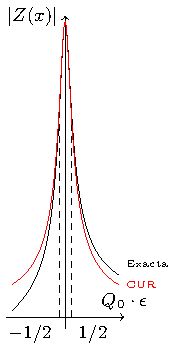
\includegraphics[height=4cm]{../figs/CUR.pdf}
\end{center}


{Puntos de potencia mitad en la CUR}



\begin{itemize}
\item La Curva Universal de Resonancia es simétrica: la frecuencia de resonancia está en el centro del ancho de banda.
\item Retomamos la expresión aproximada de los puntos de potencia mitad:
\end{itemize}
\[
  \omega_{1,2} \simeq \omega_0 (1 \mp \frac{1}{2Q_0})
\]


\begin{center}
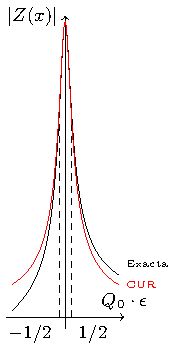
\includegraphics[height=4cm]{../figs/CUR.pdf}
\end{center}


\begin{itemize}
\item Reescribimos usando la desintonización relativa:
\end{itemize}
\[
  \frac{\omega_{1,2} - \omega_0}{\omega_0} \simeq \mp \frac{1}{2Q_0}
\]

\[
  \boxed{x_{1,2} = Q_0 \cdot \epsilon_{1,2} = \mp \frac{1}{2}} \rightarrow Z(x_{1,2}) = \frac{1}{\sqrt{2}}
\]


\subsection{Circuito RLC serie}
\label{sec:org3edc28d}
{Impedancia}

\begin{itemize}
\item Impedancia
\end{itemize}
\[
  \fasor{Z} = R + j(\omega L - \frac{1}{\omega C})
\]
\begin{itemize}
\item Impedancia en función de \(\omega_0\) y \(Q_0\)
\end{itemize}
\[
  \fasor{Z} = R \left[1 + j Q_0 \left(\frac{\omega}{\omega_0} - \frac{\omega_0}{\omega}\right)\right]
\]

\begin{itemize}
\item Impedancia en función de la desintonización relativa
\end{itemize}
\[
  \fasor{Z} = Z_0 \left[ 1 + j Q_0 \epsilon\left(\frac{2 + \epsilon}{1 + \epsilon}\right)\right]
\]  

{Frecuencias}

\begin{itemize}
\item Pulsación de Resonancia
\end{itemize}
\[
  \omega_0 = \frac{1}{\sqrt{LC}}
\]
\begin{itemize}
\item Puntos de Potencia Mitad
\end{itemize}
\[
\omega_{1,2}= \mp \frac{R}{2L} + \sqrt{\left(\frac{R}{2L}\right)^2 + \frac{1}{LC}}
\]

\begin{itemize}
\item Ancho de Banda
\end{itemize}
\[
B = \omega_2 - \omega_1 = \frac{R}{L}
\]

\begin{itemize}
\item Factor de Calidad
\end{itemize}
\[
  Q_0 = \frac{1}{\omega_0 C R} = \frac{\omega_0 L}{R}
\]

{Tensiones y energías}


\begin{itemize}
\item Tensiones en los elementos
\end{itemize}

\begin{align*}
  U(\omega_0) &= U_R(\omega_0)\\
  U_L(\omega_0) &= U_C(\omega_0) = Q_0 U
\end{align*}

\begin{itemize}
\item Energías almacenadas
\end{itemize}

\begin{align*}
  w_L(t) + w_c(t) &= \frac{1}{2} L I_0^2\\
  P_R &= R I^2\\
  w_{total} &= \frac{Q_0}{2\pi} w_R
\end{align*}

{Curva Universal de Resonancia}

\begin{itemize}
\item Aproximación para cercanías de la resonancia
\end{itemize}
\[
  \fasor{Z} \simeq Z_0 (1 + j 2 Q_0 \epsilon)
\]

\[
  |\fasor{Z}| \simeq Z_0 \sqrt{1 + 4 Q^2_0 \epsilon^2}
\]
\begin{itemize}
\item Curva Universal de Resonancia
\end{itemize}
\[
  Y(x) = \frac{1}{\sqrt{1 + 4 x^2}}
\]
\subsection{Otros circuitos}
\label{sec:org02b2019}

\subsubsection{Circuito RLC con bobina real}
\label{sec:orgfc5a9de}
\begin{center}
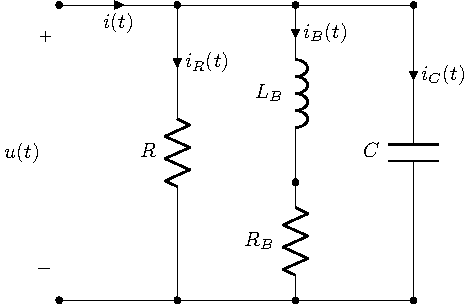
\includegraphics[height=4cm]{../figs/resonante_real.pdf}
\end{center}

La figura representa un circuito paralelo con una bobina real (con pérdidas). La impedancia de este circuito es:
\begin{align*}
\fasor{Y} &= \frac{1}{R} + j \omega C + \frac{1}{R_B + j \omega L_B} = \\ 
          &= \left(\frac{1}{R} + \frac{R_B}{R_B^2 + \omega^2 L_B^2}\right) + j \left(\omega C - \frac{\omega L_B}{R_B^2 + \omega^2 L_B^2}\right)
\end{align*}

{Impedancia}


\[
\fasor{Y} = \left(\frac{1}{R} + \frac{R_B}{R_B^2 + \omega^2 L_B^2}\right) + j \left(\omega C - \frac{\omega L_B}{R_B^2 + \omega^2 L_B^2}\right)
\]
\begin{itemize}
\item Condición de Resonancia
\end{itemize}
\[
  \omega C - \frac{\omega L_B}{R_B^2 + \omega^2 L_B^2} = 0 
\]

\begin{itemize}
\item Pulsación de Resonancia
\end{itemize}
\[
\omega_0 = \sqrt{\frac{1}{L_BC} - \left(\frac{R_B}{L_B}\right)^2}
\]
{Comparación con RLC paralelo}

\begin{itemize}
\item La frecuencia de resonancia es diferente a un RLC serie/paralelo:
\end{itemize}

\[
\omega_0 \neq \frac{1}{\sqrt{LC}}
\]

\begin{itemize}
\item El valor máximo de la admitancia \textbf{no} se alcanza en la frecuencia de resonancia, \(\omega_{max} \neq \omega_0\).

\item Cuando la \textbf{bobina} tiene \textbf{bajas pérdidas (Q alto)}, el circuito puede simplificarse a un RLC paralelo.
\end{itemize}
\subsection{Factor de Calidad de Componentes}

{Factor de Calidad}

\begin{itemize}
\item Retomamos la definición del factor de calidad como ratio entre la \textbf{máxima energía almacenada} y la \textbf{energía disipada en un período}.
\end{itemize}

\[
  Q(\omega) = 2\pi \frac{\max\{w_x(t)\}}{T \cdot P_R}
\]

{Bobina Real}

\begin{itemize}
\item Una bobina real tiene pérdidas resistivas debidas al hilo conductor\footnote{En algunos textos se emplea la tangente de pérdidas para caracterizar a la bobina real, siendo \(\tan{\delta} = 1/Q\).}.
\item Se modela como una conexión serie de una bobina ideal y una resistencia.
\end{itemize}
\begin{center}
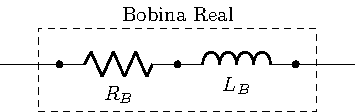
\includegraphics[height=4cm]{../figs/BobinaReal.pdf}
\end{center}

\[
  \left.
  \begin{array}{l}
    \max\{w_L(t)\} = \frac{1}{2} L_B I_o^2 = L_BI^2\\
      p_R(t) = R_B I^2
  \end{array}
  \right\} \rightarrow
  \boxed{Q(\omega) = \frac{\omega L_B}{R_B}}
\]
{Condensador Real}

\begin{center}
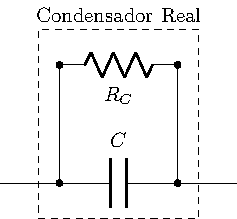
\includegraphics[height=4cm]{../figs/CondensadorReal.pdf}
\end{center}

\[
  \left.
  \begin{array}{l}
    \max\{w_C(t)\} = \frac{1}{2} C U_o^2 = CU^2\\
      p_R(t) = G_C U^2
  \end{array}
  \right\} \rightarrow
  \boxed{Q(\omega) = \omega C R_C}
\]
{Ejercicio}

Demuestra que la expresión del factor de calidad de una bobina con pérdidas modelada como un circuito paralelo es:
\begin{enumerate}
\item \hfill{}\textsc{BMCOL}
\label{sec:org17041f7}
\[
\boxed{Q = \frac{R_B}{\omega L_B}}
\]
\item \hfill{}\textsc{BMCOL}
\label{sec:orgf1bcb03}
\begin{center}
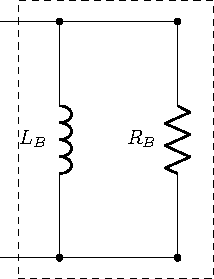
\includegraphics[height=4cm]{../figs/BobinaRealParalelo.pdf}
\end{center}
\end{enumerate}


{Conversión serie-paralelo}

\[
  \fasor{Y_s} = \frac{R_s - j\omega L_s}{R_s^2 + (\omega L_s)^2}
\]
\begin{center}
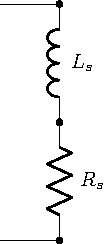
\includegraphics[height=4cm]{../figs/BobinaSerie.pdf}
\end{center}


\[
  \fasor{Y_p} = \frac{1}{R_p} - j\frac{1}{\omega L_p}
\]
\begin{center}
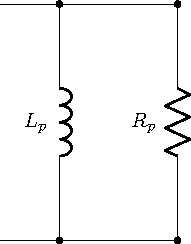
\includegraphics[height=4cm]{../figs/BobinaParalelo.pdf}
\end{center}


\[
\left.
\begin{array}{l}
  R_p = \frac{R_s^2 + (\omega L_s)^2}{R_s}\\
  \omega L_p = \frac{R_s^2 + (\omega L_s)^2}{\omega L_s}
\end{array}
\right\} \Rightarrow
\frac{\omega L_s}{R_s} = \frac{R_p}{\omega L_p} \Rightarrow \boxed{Q_p = Q_s}
\]


{Conversión serie-paralelo}
\[
  \begin{array}{l}
      R_p = R_s + \frac{(\omega L_s)^2}{R_s} \xrightarrow{\omega L_s= Q_s \cdot R_s} \boxed{R_p = R_s ( 1 + Q_S^2)}\\
      \omega L_p = \omega L_s + \frac{R_s^2}{\omega L_s} \xrightarrow{R_s = \omega L_s/Q_s} \boxed{L_p = L_s (1 + 1/Q_s^2)}
  \end{array}
\]

Para bobinas con alto factor de calidad (\(Q \geq 10\))

\begin{center}
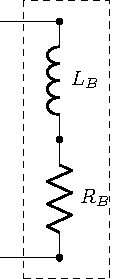
\includegraphics[height=4cm]{../figs/BobinaReal2.pdf}
\end{center}

\[
\boxed{
\begin{array}{l}
  R_p \simeq Q^2 \cdot R_s\\
  L_p \simeq L_s
\end{array}}
\]


\begin{center}
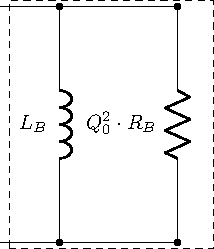
\includegraphics[height=4cm]{../figs/RL_paralelo.pdf}
\end{center}

{Conversión Serie-Paralelo}

Empleando ecuaciones similares se puede demostrar la siguiente transformación para un condensador de alto factor de calidad:
\begin{enumerate}
\item \hfill{}\textsc{BMCOL}
\label{sec:org1ccb5ad}
\begin{center}
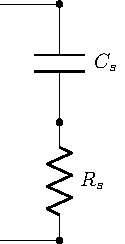
\includegraphics[height=4cm]{../figs/CondensadorSerie.pdf}
\end{center}
\item \hfill{}\textsc{BMCOL}
\label{sec:org4c6472c}
\[
\boxed{
\begin{array}{l}
  R_p \simeq Q^2 \cdot R_s\\
  C_p \simeq C_s
\end{array}}
\]

\item \hfill{}\textsc{BMCOL}
\label{sec:org7c245a2}
\begin{center}
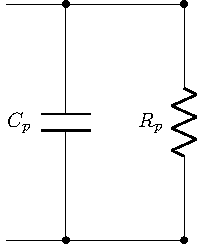
\includegraphics[height=4cm]{../figs/CondensadorParalelo.pdf}
\end{center}
\end{enumerate}

{Aplicación: transformación de circuito RLC}

\begin{center}
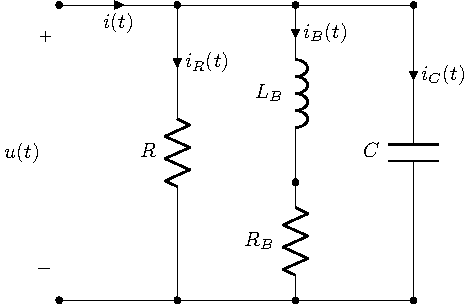
\includegraphics[height=4cm]{../figs/resonante_real.pdf}
\end{center}

\subsubsection{Ejercicios Recomendados}
\label{sec:orgc1d6688}
\begin{itemize}
\item AS: ejemplos 14.7 y 14.8
\item HKD: página 641 (voltímetro), y práctica 16.8
\item PO: problemas 23.5 y 23.7
\end{itemize}

%%% Local Variables:
%%% mode: latex
%%% TeX-master: "TC"
%%% ispell-local-dictionary: "castellano"
%%% End:
